\documentclass[aspectratio=169,11pt,table]{beamer}
\usepackage{../assets/ccde-beamer}

% ---------- Metadatos canónicos CCDE (Sin fecha por norma institucional) ----------
\renewcommand{\ccdefootlabel}{CCDE -- Dinámica de Pobreza y Vulnerabilidad}

\title{Modelado Econométrico y Machine Learning para la Vulnerabilidad y Dinámica de Pobreza}
\subtitle{Evaluación comparativa con microdatos panel ENAHO (Perú)}
\author{Círculo de Ciencia de Datos y Econometría}
\date{}

\begin{document}

% Portada canónica CCDE
\ccdeportada{Vulnerabilidad y Dinámica de Pobreza}{Logit Multinomial Clustered vs. Ensambles ML (ENAHO)}{CCDE}

% Frame 1: Agenda
\begin{frame}{Mapa de la presentación}
\begin{columns}[T,onlytextwidth]
\begin{column}{0.54\textwidth}
\small
\tableofcontents
\end{column}
\begin{column}{0.43\textwidth}
\begin{keybox}
\textbf{Pregunta guía}\par\vspace{0.10cm}
¿Cómo modelar la transición entre estados de pobreza superando el riesgo de fuga de datos (\textit{data leakage}) y qué valor añaden los ensambles frente a la econometría clásica?
\end{keybox}
\vspace{0.14cm}
\begin{ccdebox}
\small
\textbf{Población analizada:}\\
Panel ENAHO (INEI Perú), $N = 37{,}985$ hogares.\\[0.10cm]
\textbf{Modelos comparados:}\\
Logit Multinomial Clustered, Regresión Logística L2, Random Forest y Gradient Boosting.
\end{ccdebox}
\end{column}
\end{columns}
\end{frame}

\section{Fundamentos Metodológicos}

% Frame 2: Definición del Target y Clases
\begin{frame}{Definición de Estados de Vulnerabilidad}
\begin{columns}[T,onlytextwidth]
\begin{column}{0.48\textwidth}
\begin{ccdebox}
\textbf{Estados Dinámicos del Hogar ($Y$)}\par\vspace{0.10cm}
A partir del seguimiento temporal panel de la ENAHO, se definen 4 categorías:
\begin{itemize}
    \item \textbf{0. Resiliente:} No pobre en $t$ y no pobre en $t+1$ ($N=27{,}975$).
    \item \textbf{1. Cae en pobreza:} Vulnerable que transita a la pobreza ($N=2{,}729$).
    \item \textbf{2. Sale de pobreza:} Hogar en recuperación transitoria ($N=3{,}081$).
    \item \textbf{3. Pobre crónico:} Permanece bajo la línea en ambos periodos ($N=4{,}200$).
\end{itemize}
\end{ccdebox}
\end{column}
\begin{column}{0.48\textwidth}
\begin{contrastbox}{warn}{El Reto Metodológico: Data Leakage}
\begin{itemize}
    \item Los ratios directos con la línea de pobreza ($gasto/línea$) generan \textit{separación casi perfecta} en modelos multinomiales.
    \item \textbf{Estrategia en la rama avances-abel:}
    \begin{enumerate}
        \item \textit{MNLogit:} variables demográficas y logaritmos de ingreso/gasto con errores agrupados por conglomerado.
        \item \textit{Modelos ML:} exploración completa de proximidad a la línea con validación estratificada ($K=5$).
    \end{enumerate}
\end{itemize}
\end{contrastbox}
\end{column}
\end{columns}
\source{Elaboración CCDE con microdatos ENAHO (INEI)}
\end{frame}

\section{Resultados Empíricos}

% Frame 3: Tabla Comparativa
\begin{frame}{Rendimiento Comparativo de Modelos}
\begin{columns}[T,onlytextwidth]
\begin{column}{0.54\textwidth}
\begin{table}
\centering
\small
\begin{tabular}{lcc}
\hline
\textbf{Modelo} & \textbf{F1 Macro} & \textbf{F1 Weighted} \\
\hline
Regresión Logística (L2) & 0.5427 & 0.8191 \\
Gradient Boosting        & 0.5817 & \textbf{0.8314} \\
Random Forest (Ensambles) & \textbf{0.6081} & 0.7578 \\
\hline
\end{tabular}
\end{table}
\vspace{0.15cm}
\begin{keybox}
\textbf{Hallazgo Clave}\par\vspace{0.08cm}
Random Forest logra el mayor balance entre clases con un \textbf{F1-Macro de 0.6081}, capturando no linealidades de hogares en transición. Gradient Boosting maximiza la exactitud global ponderada (\textbf{0.8314}).
\end{keybox}
\end{column}
\begin{column}{0.43\textwidth}
\begin{ccdebox}
\textbf{Diagnóstico de Clasificación}\par\vspace{0.10cm}
\begin{itemize}
    \item La clase \textbf{Resiliente} se predice con precisión superior al $91\%$.
    \item La dificultad analítica radica en distinguir entre \textit{Salir de pobreza} vs. \textit{Pobreza crónica}, debido a la volatilidad de ingresos informales alrededor de la línea.
\end{itemize}
\end{ccdebox}
\end{column}
\end{columns}
\source{Validación cruzada estratificada $K=5$, rama: avances-abel}
\end{frame}

% Frame 4: Importancia de Variables
\begin{frame}{Importancia de Factores de Vulnerabilidad (Random Forest)}
\begin{columns}[c,onlytextwidth]
\begin{column}{0.50\textwidth}
\centering
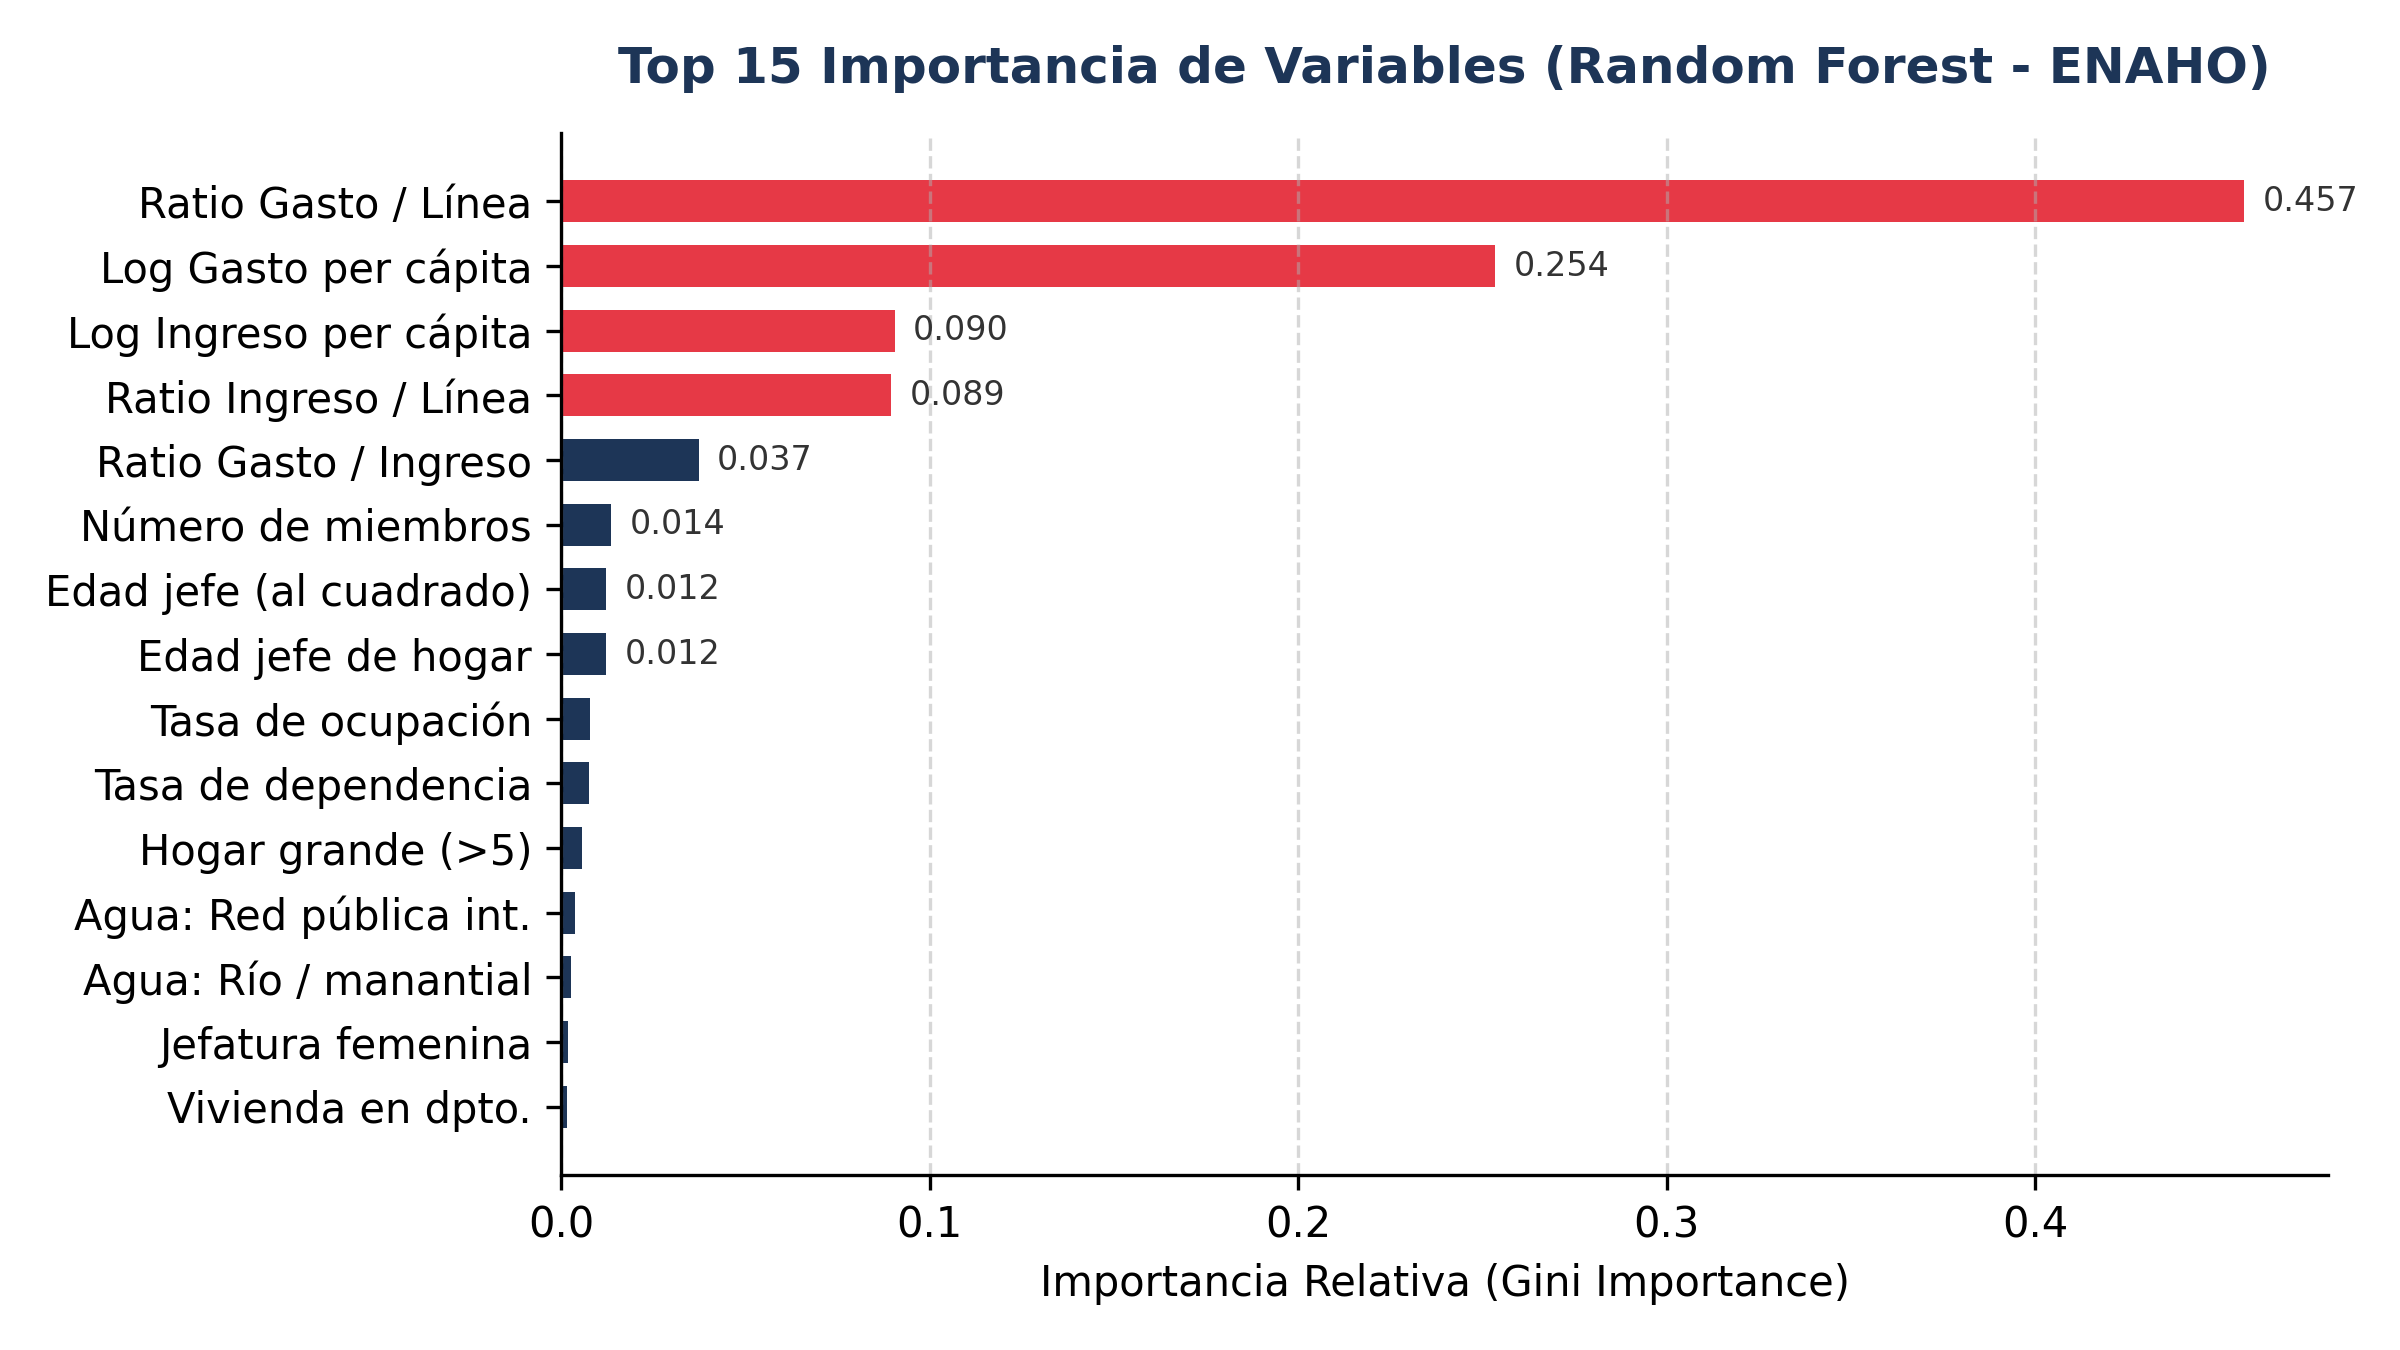
\includegraphics[width=\textwidth]{fig_importancia_rf.png}
\end{column}
\begin{column}{0.47\textwidth}
\begin{ccdebox}
\textbf{Drivers Estructurales Determinantes}\par\vspace{0.08cm}
\begin{enumerate}
    \item \textbf{Cojín de consumo ($0.457$):} La holgura del gasto frente a la canasta básica es el primer escudo contra shocks.
    \item \textbf{Nivel per cápita ($0.254$):} Magnitud absoluta de ingresos y gastos.
    \item \textbf{Carga demográfica:} Número de miembros ($1.36\%$), edad del jefe y tasa de ocupación laboral.
    \item \textbf{Acceso a servicios:} Cobertura de red de agua potable vs. fuentes precarias.
\end{enumerate}
\end{ccdebox}
\end{column}
\end{columns}
\source{Random Forest Classifier ($100$ estimadores, $N=37{,}985$)}
\end{frame}

\section{Conclusiones y Recomendaciones}

% Frame 5: Conclusiones
\begin{frame}{Conclusiones y Política Pública Focalizada}
\begin{columns}[T,onlytextwidth]
\begin{column}{0.48\textwidth}
\begin{keybox}
\textbf{Aporte Metodológico}\par\vspace{0.08cm}
La combinación de modelación econométrica (controlando por heterogeneidad con conglomerados) y ensambles ML permite identificar el umbral crítico donde un shock transitorio empuja al hogar a la pobreza crónica.
\end{keybox}
\end{column}
\begin{column}{0.48\textwidth}
\begin{contrastbox}{ccdeblue}{Implicancia de Política}
Las políticas de transferencias y programas de alivio no deben fijarse exclusivamente en el estado de pobreza estático, sino en el gradiente de vulnerabilidad predicho para prevenir transiciones antes de que se vuelvan crónicas.
\end{contrastbox}
\end{column}
\end{columns}
\vspace{0.25cm}
\begin{ccdebox}
\small
\textbf{Código y Reproducibilidad:}\\
Pipeline desarrollado bajo especificación de producción en \texttt{vulnerabilidad-hogares} (\texttt{src/explotando\_modelo.py}).
\end{ccdebox}
\end{frame}

\end{document}
